\documentclass[../ana1.tex]{subfiles}
\onlyinsubfile{\sectionNumbering} %Use numbering relative to sections and not subsection

\begin{document}
\setcounter{section}{16}
\section{Eigenschaften stetiger Funktionen}
\begin{defi}[Gleichmäßige Stetigkeit]
    Eine Funktion \( f: D \rightarrow \C \) 
    heißt gleichmäßig stetig, falls
    \[ \forall \, \varepsilon > 0 \,\exists \, 
    \delta > 0 \,\forall \, z_1, z_2 \in D \text{ mit } 
    \abs{z_1 - z_2} < \delta \Rightarrow 
    \abs{f(z_1) - f(z_2)} < \varepsilon. \]
\end{defi}
\begin{bem}
    Beachte: \( \delta \) hängt nun von \(\varepsilon \) ab.
\end{bem}
\begin{bspe}\leavevmode
    \begin{enumerate}
        \item \( f: (0,1] \rightarrow \R, 
        x \mapsto \frac{1}{x} \) ist stetig in jedem 
        \( x_0 \in (0,1]. \) \\
        Wähle \( \delta := 
        \min(\frac{x_0}{2}, \frac{x_0^2 \varepsilon}{2}) \).
        Dann gilt: \( \abs{f(x) - f(x_0)} 
        \leq \frac{ 2 \abs{x-x_0} }{ x_0^2 } < \varepsilon \).\\
        Man sieht, dass das benutzte \( \delta \) umso
        kleiner wird, je mehr man sich dem linken Rand
        von \( (0,1] \) annähert.\\
        \begin{center}
            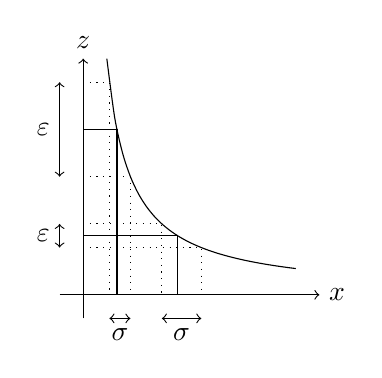
\begin{tikzpicture}[scale = 3]
                \draw[->] (0,-0.1) -- (0,1) node[above] {\(z\)};
                \draw[->] (-0.1,0) -- (1,0) node[right] {\(x\)};
                \draw[thin,domain=0.1:0.9,smooth,variable=\x,black] plot ({\x},{1 / (10 * \x)});
                \draw[dotted] (0,0.9) -- (0.111,0.9) -- (0.111,0);
                \draw[dotted] (0,0.5) -- (0.2,0.5) -- (0.2,0);
                \draw (0,0.7) -- (0.1429,0.7) -- (0.1429,0);
                \draw[<->] (-0.1,0.5) -- (-0.1,0.9) node[midway, left] {\( \varepsilon \)};
                \draw[<->] (0.111,-0.1) -- (0.2,-0.1) node[midway, below] {\(\sigma \)};

                \draw[dotted] (0,0.3) -- (0.333,0.3) -- (0.333,0);
                \draw[dotted] (0,0.2) -- (0.5,0.2) -- (0.5,0);
                \draw (0,0.25) -- (0.4,0.25) -- (0.4,0);
                \draw[<->] (-0.1,0.2) -- (-0.1,0.3) node[midway, left] {\( \varepsilon \)};
                \draw[<->] (0.333,-0.1) -- (0.5,-0.1) node[midway, below] {\(\sigma \)};

            \end{tikzpicture}
        \end{center}
        \( f \) ist nicht gleichmäßig stetig in \( (0,1] \),
        da man \( \delta \) nicht unabhängig von \(x\) wählen
        kann.\\
        Wäre \( f \) gleichmäßig stetig, so könnte man zu 
        \( \varepsilon = 1 \) ein \( \delta > 0 \) wählen,
        sodass \( \abs{ f(x) - f(\tilde{x}) } < 1 
        \,\forall \, x, \tilde{x} \in (0,1] \) mit 
        \( \abs{ x - \tilde{x} } < \delta (*) \).\\
        Es gibt aber ein \( n \geq 1 \) mit 
        \( \abs{ \frac{1}{n} - \frac{1}{2n} } < \delta \)
        und \( \abs{ f(\frac{1}{n}) - f(\frac{1}{2n}) } 
        = n \geq 1 \).
        \item Jede gleichmäßig stetige Funktion ist stetig.
        \item \( f: \R \rightarrow \R, x\mapsto x^2 \) ist stetig,
        aber nicht gleichmäßig stetig. 
        Aber \( g: [-1, 1] \rightarrow \R, x \mapsto x^2 \)
        ist gleichmäßig stetig.
    \end{enumerate}
\end{bspe}
\begin{satz}[Satz von Heine]
    Sei \( D \subset \C \) abgeschlossen und beschränkt
    und \( f: D \rightarrow \C \) stetig.\\
    Dann ist \(f\) gleichmäßig stetig.
\end{satz}
\begin{bew}
    Angenommen \(D\) ist abgeschlossen und beschränkt und
    \( f: D \rightarrow \C \) ist stetig, aber nicht gleichmäßig
    stetig (\( \leadsto \) Widerspruch)\\
    \( f \) nicht gleichmäßig stetig heißt:
    \[ \exists \, \varepsilon > 0 \,\forall \, 
    \delta > 0 \,\exists \, u, w \in D: \abs{u-w}
    < \delta \text{ und } \abs{f(u) - f(w)} \geq \varepsilon \]
    Wähle \( n\in\N, \delta = \frac{1}{n} \). Das heißt, 
    es gibt \( {(x_n)}_n, {(y_n)}_n \subseteq D \) mit 
    \( \abs{x_n - y_n} < \frac{1}{n} \) und 
    \( \abs{f(x_n) - f(y_n)} \geq \varepsilon \) für 
    \( n\in\N \).\\
    Da \( {(y_n)}_n \subseteq D \) und \( D \) beschränkt ist,
    existiert eine konvergente Teilfolge von \( {(y_n)}_n \).
    \( \exists \, \sigma : \N \rightarrow \N,
    \sigma(n) < \sigma(n+1) \,\forall \, n\in\N \), 
    sodass \( y_{\sigma(k)} \) konvergiert.\\
    \( z_0 := \limes{k} y_{\sigma(k)} \). Da \(D\) abgeschlossen
    ist und \( y_{\sigma(k)} \in D \,\forall \, k \in\N \), 
    ist \( z_0 \in D \).\\
    Betrachte Teilfolge \( \tilde{x}_k := x_{\sigma(k)} \).
    Dann gilt:
    \[ \abs{ \tilde{x}_k - y_{\sigma(k)} } 
    = \abs{ x_{\sigma(k)} - y_{\sigma(k)} }
    < \frac{1}{\sigma(k)} \rightarrow 0. \]
    Da \( y_{\sigma(k)} \rightarrow z_0 \), folgt 
    \( \abs{ \tilde{x}_k - z_0 } \rightarrow 0. \) \\
    Also \( \limes{k} \tilde{x}_k = z_0 \) und 
    \begin{align*}
        \varepsilon \leq &\abs{ f(x_{\sigma(k)}) - f(y_{\sigma(k)}) }\\
        = &\abs{ f(x_{\sigma(k)}) - f(z_0) + f(z_0) - f(y_{\sigma(k)}) }\\
        \leq &\abs{ f(x_{\sigma(k)}) - f(z_0) } + \underbrace{\abs{ f(z_0) - f(y_{\sigma(k)}) }}_{\longrightarrow 0}
    \end{align*}
    Es ist also 
    \[ \limesinf{k} \abs{ f(x_{\sigma(k)}) - f(z_0) } \geq \varepsilon > 0 \text{ \Lightning{} zu Stetigkeit von  } f \text{ in } x_0. \]
\end{bew}
\begin{bem}
    Alle Polynome, \( \exp, \sin, \cos \) sind somit
    auf abgeschlossenen und beschränkten Teilmengen
    von \( \C \) gleichmäßig stetig. Insbesondere 
    gilt dies auf allen Intervallen \( [a,b], 
    a<b \in\R \).
\end{bem}
\begin{defi}[Folgenkompaktheit]
    Sei \( D \subset \R \) oder \( D \subset \C \)
    heißt folgenkompakt oder einfach kompakt, wenn
    jede Folge \( {(a_n)}_n \subset D \) eine
    konvergente Teilfolge \( {(a_{\sigma(n)})}_n \)
    besitzt mit \( \limes{n} a_{\sigma(n)} \in D \), 
    wobei \( \sigma : \N \rightarrow \N \) eine 
    Verdünnung ist.
\end{defi}
\begin{satz}[Heine-Borel]
    \( D \subset \C \) ist beschränkt und abgeschlossen, 
    wenn \( {(z_n)}_n \subset D \) eine konvergente
    Teilfolge besitzt, deren Grenzwert wieder in 
    \( D \) liegt.
\end{satz}
\begin{bew}
    \equirl{
        Sei \( D \subset \C \) beschränkt und 
        abgeschlossen und \( {(a_n)}_n \subset D \) 
        Folge in \( D \). Nach dem Satz von 
        Bolzano-Weierstraß besitzt \( {(a_n)}_n \)
        eine konvergente Teilfolge. Diese konvergiert, 
        da \( D \) abgeschlossen ist, gegen einen Wert 
        aus \( D \).\\
        Also ist \( D \) folgenkompakt.
    }{
        Sei \( D \) folgenkompakt.\\
        Zur Beschränktheit: Nehmen an, dass \( D \) 
        unbeschränkt ist. Sei \( {(a_n)}_n \) eine 
        Folge mit \( a_1 \in D \) und \( \abs{a_{n+1}} 
        > \abs{a_n} + 1 \) für \( n\in\N \). Dann 
        besitzt \( {(a_n)}_n \) keine konvergente 
        Teilfolge, da
        \[ \abs{ a_{n+1} - a_n } \geq 1 
        \;\forall \, n\in\N. \]
        Dies widerspricht der Folgenkompaktheit von
        \( D \).\\
        Zur Abgeschlossenheit: Da jede Teilfolge einer 
        konvergenten Folge \( {(a_n)}_n \) mit demselben
        Grenzwert konvergiert, muss dieser in \( D \)
        liegen.
    }
\end{bew}
\begin{satz}[Vom Minimum und Maximum]
    Sei \( D \subset \C \) abgeschlossen und 
    beschränkt und \( f : D \rightarrow \R \) eine
    stetige Funktion.\\
    Dann nimmt \(f\) sein Minimum und sein Maximum 
    auf \(D\) an, d.\ h.\ es gibt ein \( z_{\min} \)
    und \( z_{\max} \) mit
    \begin{align*}
        f(z_{\min}) &= \inf f(D) &= \min f(D) \\
        f(z_{\max}) &= \sup f(D) &= \max f(D)
    \end{align*}
    Insbesondere gilt 
    \[ \abs{f(z)} \leq \max ( \abs{ f(z_{\min)} }, 
    \abs{ f(z_{\max}) } ) \; \forall \, z\in D. \]
\end{satz}
\begin{bew}\leavevmode \\
    Teil 1: \(f\) ist beschränkt.\\
    Angenommen, \(f\) ist unbeschränkt. D.\ h.\ für 
    alle \( k>0 \) existiert \( z\in D \), sodass
    \( \abs{f(z)} > k \). Wähle \( k=n \). \\
    Dann existiert eine Folge \( {(z_n)}_n \subset D \),
    sodass \( \abs{f(z_n)} > n \).\\
    Da \( {(z_n)}_n \subset D \) und \(D\) kompakt ist, 
    gibt es eine konvergente Teilfolge 
    \( {(z_{\sigma(n)})}_n \subset D \) von 
    \( {(z_n)}_n \subset D \).\\
    Wir setzen \( z_0 := \limes{n} z_{\sigma(n)} 
    \in D \). Dann gilt 
    \[ \abs{f(z_{\sigma(n)})} > \sigma(n) \geq n 
    \;\forall \, n\in\N. \]
    Da \(f\) stetig ist, gilt \( f(z_{\sigma(n)}) 
    \overset{n\rightarrow\infty}{\longrightarrow}
    f(z_0) \) \Lightning{} d.\ h.\  \(f\) muss 
    beschränkt sein auf \(D\).\\
    Teil 2: Es gibt \( z_{\min} \in D \) mit 
    \( f(z_{\min}) = \inf \Bild(f) \).\\
    \[ \text{Es gilt } \alpha_+, \alpha_{\minus} 
    \in \R .\]
    Da \( \alpha_{\minus} \) größte untere Schranke 
    von \( \Bild(f) \) ist, ist für alle \( n\in\N 
    \alpha_{\minus} + \frac{1}{n} \) keine untere 
    Schranke von \( \Bild(f) \). Für alle 
    \( n\in\N \) gibt es \( {(z_n)}_n \subset D \), 
    sodass 
    \[ f(z_n) \leq \alpha_{\minus} + \frac{1}{n}. \]
    Da \( \alpha_{\minus} \leq f(z) \) für 
    \( z\in D \), wissen wir
    \[ \alpha_{\minus} \leq f(z_n) \leq 
    \alpha_{\minus} + \frac{1}{n}. \]
    Nach dem Sandwichkriterium gilt also 
    \[ \limes{n} f(z_n) = \alpha_{\minus}. \]
    %BEMERKUNG?
    Da \(D\) kompakt ist, gibt es eine konvergente 
    Teilfolge \( {(z_{\sigma(n)})}_n \) von 
    \( {(z_n)}_n \) mit \( \sigma : \N 
    \rightarrow \N \) mit \( \sigma(n+1) \geq 
    \sigma(n) \) für alle \( n\in\N \), deren Grenzwert 
    in \(D\) liegt.\\
    Setzen \( z_{\min} := \limes{n} z_{\sigma(n)} \). 
    Dann gilt wegen der Stetigkeit von \(f\)
    \[ f(z_{\min}) = \limes{n} f(z_{\sigma(n)}) 
    = \alpha_{\minus} = \inf f(D). \]
    Für das Maximum geht man analog vor.
\end{bew}
\begin{defi}[Stetige Fortsetzung]
    Es sei \( D \subset \C \) nicht abgeschlossen, 
    \( f: D\rightarrow \C \) und \( z_0 \in \bar{D}
    \setminus D \) und \( w_0 \in \C \) seien gegeben.\\
    Wenn Grenzwert \( \limesx{z}{z_0} f(z) = w_0 \)
    existiert, dann heißt die Funktion 
    \[ \bar{f} : \bar{D} := D \cup \set{z_0} 
    \rightarrow \C \]
    \[ \bar{f}(z) := 
    \begin{cases}
        f(z), &z\in D \\
        w_0, &z = z_0
    \end{cases} \]
    stetige Fortsetzung von \(f\) auf \(z_0\).
\end{defi}
\begin{bspe}\leavevmode
    \begin{enumerate}
        \item \[ D = \R \setminus \set{1}, 
        f(x) = \frac{x^2 - 1}{x - 1}, x\in D, \]
        dann wird \(f\) durch
        \[ \bar{f}(x) := 
        \begin{cases}
            \frac{x^2 - 1}{x - 1}, &x\neq 1\\
            2, &x = 1
        \end{cases} (=x+1) \]
        stetig fortgesetzt.
        \item \( D \in\R\setminus \set{0} \). Die 
        Funktionen \( f: D \rightarrow \R, 
        x\mapsto \frac{1}{x} \) und \( g: D 
        \rightarrow \R, x \mapsto 
        \mathds{1}_{(0,\infty)}(x) \) nicht stetig 
        fortsetzbar in \(0\).
    \end{enumerate}
\end{bspe}
\begin{satz}
    Sei \( f: D\rightarrow \C \) gleichmäßig stetig. 
    Dann hat \(f\) eine eindeutige stetige Fortsetzung 
    \( \bar{f} : \bar{D} \rightarrow \C \). Diese ist 
    auch gleichmäßig stetig.
\end{satz}
\begin{bew}
    Eindeutigkeit: Seien \( h_1,h_2 : \bar{D} 
    \rightarrow \C \) zwei Fortsetzungen von 
    \( f : D \rightarrow \C \). Betrachte 
    \[ g: \bar{D} \rightarrow \C, z \mapsto 
    h_1(z) - h_2(z). \]
    Dann ist \(g\) stetig und \( g(z) = 0 
    \, \forall z\in D \).\\
    Damit \( g(z) = 0 \,\forall \, z \in D \), da für 
    \( \bar{D} \setminus D \) eine Folge 
    \( {(z_n)}_n \subset D \) existiert mit 
    \( \limes{n} z_n = z \) und somit 
    \[ g(z) = g(\limes{n} z_n) = \limes{n} g(z_n) = 0 \]
    wegen der Stetigkeit von \(g\) und \( g=0 \) auf \(D\).\\
    Existenz: Wir definieren \( \bar{f}: \bar{D} 
    \rightarrow \C \) durch:\\
    Ist \( z\in D \), dann ist \( \bar{f}(z) = f(z) \).\\
    Ist \( z\in \bar{D}\setminus D \), dann existiert
    eine Folge \( {(z_n)}_n \subset D \) mit 
    \( \limes{n} z_n = z \). Wir setzen \( \bar{f}(z) 
    = \limes{n} f(z_n) \).\\
    Aber wir wissen noch nicht, dass dieser Grenzwert 
    existiert. Da \(z_n \rightarrow z\) für 
    \(n\rightarrow \infty \), ist \( {(z_n)}_n \) eine 
    Cauchy-Folge.\\
    Beh.\ 1: \( {(f(z_n))}_n \) ist Cauchy-Folge.\\
    Sei \( \varepsilon > 0 \). Da \(f\) gleichmäßig stetig 
    ist, gilt 
    \[ \exists \delta > 0 : \forall \, z, w \in D 
    \text{ mit } \abs{z-w} < \delta \Rightarrow 
    \abs{f(z) - f(w)} < \varepsilon. \]
    Da \( {(z_n)}_n \) Cauchy ist, gibt es ein \( N\in\N \), 
    sodass für \( n,m\in\N \)
    \[ \abs{z_n - z_m} < \delta. \]
    D.\ h.\  \( \abs{f(z_n) - f(z_m)} < \varepsilon 
    \Rightarrow {(f(z_n))}_n \) ist Cauchy.\\
    Beh.\ 2.: Der Grenzwert von \( \limes{n} f(z_n) \)
    hängt nicht von \( {(z_n)}_n \) ab, d.\ h.\ sind 
    \( {(u_n)}_n, {(w_n)}_n \subset D \) und 
    \( w_n \rightarrow z, u_n \rightarrow z \) für 
    \(n\rightarrow \infty \). Dann gilt 
    \[ \limes{n} f(u_n) = \limes{n} f(w_n). \]
    Gilt dies, wäre die Definition \(f\) sinnvoll.\\
    Sei nun \( {(u_n)}_n, {(w_n)}_n \subset D \) mit 
    \( w_n \rightarrow z, u_n \rightarrow z \). \\
    Dann folgt für \( {(v_n)}_n \) gegeben durch 
    \( v_{2n-1} = u_n, v_{2n} - w_n \)
    \[ \limes{n} v_n = z. \]
    Wegen Beh.\ 1 existiert \( \gamma := \limes{n} f(v_n) \).\\
    Dann ist aber auch \( \limes{n} f(u_n) = \gamma 
    = \limes{n}f(w_n) \).\\
    Beh.\ 3: \( \bar{f} \) ist gleichmäßig stetig.\\
    Sei \( \varepsilon > 0 \) und \( \delta > 0 \) so, 
    dass 
    \[ \forall \, u,w\in D : \abs{u-w} < \delta 
    \Rightarrow \abs{f(u)-f(w)} < \varepsilon. \]
    Nun seien \( \bar{u}, \bar{w} \in \bar{D}, 
    \abs{\bar{u} - \bar{w}} < \delta \). Wähle 
    \( {(u_n)}_n, {(w_n)}_n \subset D \).\\
    \( u_n \rightarrow \bar{u}, w_n \rightarrow \bar{w} \). 
    Es gilt also \( \abs{u_n - w_n} < \delta \) für 
    fast alle \( n\in\N \) und somit
    \[ \abs{f(u_n) - f(w_n)} < \varepsilon 
    \text{ für fast alle } n\in\N. \]
    Da \( f(u_n) \rightarrow \bar{f}(\bar{u}) \) und 
    \( f(w_n) \rightarrow \bar{f}(\bar{w}) \), gilt
    \[ \abs{ \bar{f}(\bar{u}) - \bar{f}(\bar{w}) } 
    = \limes{n} \abs{ f(u_n) - f(w_n) } \leq \varepsilon. \]
    D.\ h.\  \( \bar{f} \) ist gleichmäßig stetig.
\end{bew}
Achtung: Man kann die Voraussetzung 
\( f: D\rightarrow \C \) gleichmäßig stetig nicht zu 
stetig abschwächen.\\
Die Funktion 
\[ f: \Q \rightarrow \R, x \mapsto f(x) = 
\begin{cases}
    -1, &x^2 < 2\\
    1, &x^2 > 2
\end{cases} \]
hat keine stetige Fortsetzung auf \( \R \).
Beachte: \( \bar{\Q} = \R \) (HA)
\begin{satz}[Zwischenwertsatz]
    Eine stetige Funktion \( f: [a,b] \rightarrow \R \) 
    nimmt jeden Wert \( \gamma \) zwischen \( f(a) \) 
    und \( f(b) \) an mindestens einer Stelle 
    \( c\in [a,b] \) an, d.\ h.\ es gibt ein 
    \( c \in [a,b] : f(c) = \gamma \).
\end{satz}
\begin{bem}
    Ist \( f(a) \neq f(b) \) und liegt \( \gamma \) strikt 
    \( f(a) \) und \( f(b) \), dann existiert 
    \( c \in (a,b) \), sodass \( f(c) = \gamma \).
\end{bem}
\begin{bew}
    HA
\end{bew}
Für den Beweis benötigt man das folgende Lemma.
\begin{lem}
    \( f: [a,b] \rightarrow \R \) stetig und 
    \( c \in [a,b] \) mit \( f(c) > 0 \). Dann existiert 
    ein \( \delta > 0 \), sodass 
    \[ \forall \, x\in [a,b] \cap \overline{B_\delta(c)} : 
    f(x) \geq \frac{f(c)}{2} \]
\end{lem}
\begin{bew}
    Wegen \( \varepsilon \)-\(\delta \)-Charakteristik der 
    Stetigkeit folgt \( \varepsilon := \frac{f(c)}{2} > 0 \) 
    die Existenz von \( \delta > 0 \)
    \[ \forall \, x\in [a,b] \cap B_\delta(c) : 
    \abs{f(x) - f(c)} \leq \varepsilon = \frac{f(c)}{2} \]
    Daraus folgt
    \begin{align*}
        f(x) &= f(c) + f(x) - f(c) \\
        &\geq f(c) + \abs{f(x) - f(c)} \\
        &\geq f(c) - \frac{f(c)}{2} \\
        &= \frac{f(c)}{2}.
    \end{align*}
\end{bew}
\begin{lem}[Nullstellensatz]
    Sei \( f : [a,b] \rightarrow \R \) stetig 
    mit \( f(a) \leq 0 \leq f(b) \). Dann existiert 
    ein \( c \in [a,b] \) mit \(f(c) = 0\), d.\ h.\ 
    \(f\) hat eine Nullstelle in \( [a,b] \).\\
    Ist \( f(a) < 0 < f(b) \), so ist \( c \in (a,b) \).
\end{lem}
\begin{bew}
    Ist \( f(a) = 0 \), so setze \( c=a \), ist \(f(b) = 0\), 
    so setze \( c=b \).\\
    O.\ B.\ d.\ A.\ ist \( f(a) < 0 < f(b) \).\\
    Sei \( C := \set{x \in [a,b] \;\vert \; f(x) < 0} \). 
    Dann ist \( C \neq \emptyset \), da \( a \in C \). 
    Ferner ist \(C\) durch \(b\) nach oben beschränkt. 
    Aus dem Vollständigkeitsaxiom folgt, dass eine reelle Zahl 
    \(c\) existiert 
    \[ c := \sup C. \]
    Ferner ist \( c \in [a,b] \).\\
    Da \( c = \sup C \), gibt es eine Folge 
    \( {(x_n)}_n \subset C \), sodass \( \limes{n} x_n = c \) 
    und da \(f\) stetig ist, gilt 
    \[ f(c) = \limes{n} \underbrace{f(x_n)}_{\leq 0} \leq 0. \]
    Also \( f(c) \leq 0 \) und somit \( c < b \).\\
    Wäre \( f(c) < 0 \), dann folgt aus Lemma 9 die 
    Existenz von \( \delta > 0 \), sodass aus \( x \in [a,b] 
    \cap [c-\delta, c+\delta] \) auch \( f(x) < 0 \) folgt.\\
    Da \( f(b) > 0 \), ist \( c + \delta < b \) und somit 
    \[ c + \delta \in (a,b) \text{ und } f(c+\delta) < 0. \]
    Damit ist \( c + \delta \in C \) und \( c < c + \delta \) 
    \Lightning{} \(c = \sup C\).\\
    Also muss \( f(c) = 0 \).
\end{bew}
Achtung: Wir benötigen hier sicherlich die Vollständigkeit von 
\( \R \), da für die stetige Funktion 
\[ f: \Q \rightarrow \set{-1, 1}, \]
\[ x \mapsto \begin{cases}
    1, &x^2 > 2 \\
    -1, &x^2 < 2
\end{cases} \]
gilt der Zwischenwertsatz nicht.
\begin{kor}
    Sei \( f: [a,b] \rightarrow \R \) stetig und 
    \( f(a) \cdot f(b) \leq 0 \), dann existiert 
    ein \( c \in [a,b] \) mit \( f(c) = 0 \).
\end{kor}
\begin{bew}
    Die Voraussetzung besagen, dass entweder 
    \( f(a) \) oder \( f(b) \) Null sind oder 
    \( f(a) \) und \( f(b) \) gegensätzliche 
    Vorzeichen haben.\\
    Es ist also \( f(a) \leq 0 \leq f(b) \) 
    oder \( f(b) \leq 0 \leq f(a) \).
    \( \overset{ZWS}{\Rightarrow} \) Behauptung.
\end{bew}
\end{document}